%%%%%%%%%%%%%%%%%%%%%%%%%%%%%%%%%%%%%%%%%%%%%%%%%%%%%%%%%%%%%%%%%%%%%%%%%%%%%%%%%%
\begin{frame}[fragile]\frametitle{}
\begin{center}
{\Large Tkinter}

\tiny{(Reference: CS2316, Fall 2016 http://cs2316.gatech.edu/slides/tkinter.pptx)}

\end{center}
\end{frame}



%%%%%%%%%%%%%%%%%%%%%%%%%%%%%%%%%%%%%%%%%%%%%%%%%%%
\begin{frame}[fragile] \frametitle{GUI: Graphical User Interface}

\adjustbox{valign=t}{
\begin{minipage}{0.45\linewidth}
\begin{itemize}
\item A way for people to interact with computer programs
\item Uses windows, icons and menus
\item Can be manipulated by a mouse and keyboard
\end{itemize}
%\begin{lstlisting}
%x = 2
%y = 3
%op1 = tf.add(x, y)
%op2 = tf.mul(x, y)
%useless = tf.mul(x, op1)
%op3 = tf.pow(op2, op1)
%with tf.Session() as sess:
%    op3 = sess.run(op3)
%
%\end{lstlisting}
\end{minipage}
}
\hfill
\adjustbox{valign=t}{
\begin{minipage}{0.45\linewidth}
\begin{center}
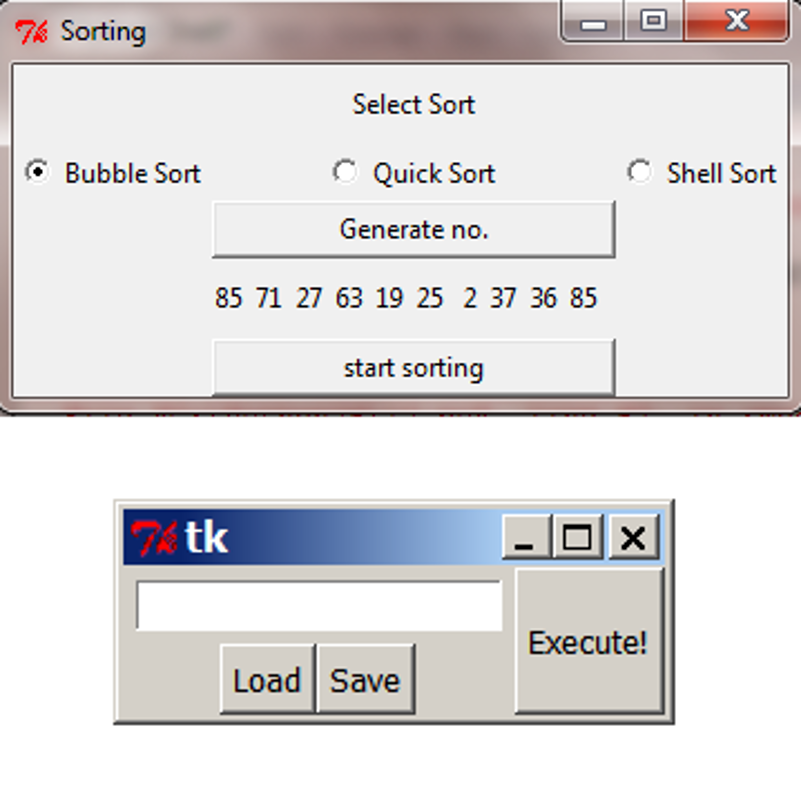
\includegraphics[width=\linewidth,keepaspectratio]{tkintergui}
\end{center}
\end{minipage}
}

\end{frame}

%%%%%%%%%%%%%%%%%%%%%%%%%%%%%%%%%%%%%%%%%%%%%%%%%%%
\begin{frame}[fragile] \frametitle{GUIs: Step by Step}
\begin{itemize}
\item Design the GUI
\item Create all the buttons, labels, entries, etc. (widgets) And specify where they go in a window
\item Write functions/methods to do what needs to be done
\item Connect the widgets to the functions/methods
\item Start the main loop
\end{itemize}
\end{frame}

%%%%%%%%%%%%%%%%%%%%%%%%%%%%%%%%%%%%%%%%%%%%%%%%%%%
\begin{frame}[fragile] \frametitle{Tkinter}
\begin{itemize}
\item Tkinter is the de facto Python standard GUI library, it comes with your installation of Python and doesn't need to be installed separately
\item We will use the Tkinter GUI toolkit to create Python GUIs \\
https://docs.python.org/3/library/tk.html 
\end{itemize}
\begin{lstlisting}
from tkinter import *
\end{lstlisting}
\end{frame}


%%%%%%%%%%%%%%%%%%%%%%%%%%%%%%%%%%%%%%%%%%%%%%%%%%%
\begin{frame}[fragile] \frametitle{Some simple tkinter widgets}

\adjustbox{valign=t}{
\begin{minipage}{0.45\linewidth}
\begin{itemize}
\item Label: Just displays text, not clickable
\item Button: Can be linked to a function/method which is called on click
\item Entry: Can allow the user to enter text, Can also be used to display text, Has 3 possible states: normal, readonly, disabled
\end{itemize}
\end{minipage}
}
\hfill
\adjustbox{valign=t}{
\begin{minipage}{0.45\linewidth}
\begin{lstlisting}
win = Tk()
win.title("My GUI")
l = Label(win, text="Hello, world")
b = Button(win, text="Click me!")
l.pack()
b.pack()

win.mainloop()
\end{lstlisting}
\begin{center}
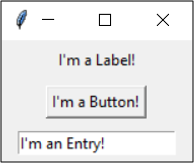
\includegraphics[width=0.5\linewidth,keepaspectratio]{tkintersimple}
\end{center}
\end{minipage}
}
This code creates a basic GUI with a Label and a Button and places them in a window using the Pack layout manager.

The button has no ``command'' so it has no function when clicked.

\end{frame}


%%%%%%%%%%%%%%%%%%%%%%%%%%%%%%%%%%%%%%%%%%%%%%%%%%%
\begin{frame}[fragile] \frametitle{Some simple tkinter widgets}

\adjustbox{valign=t}{
\begin{minipage}{0.45\linewidth}
\begin{itemize}
\item Now the clicked function will be called every time the button is clicked
\item If we defined the clicked function below the GUI code, the line creating the Button would throw a NameError
\item We can avoid this problem by writing a class for our GUI
\end{itemize}
\end{minipage}
}
\hfill
\adjustbox{valign=t}{
\begin{minipage}{0.45\linewidth}
\begin{lstlisting}
def clicked():
    print("Button clicked!")

win = Tk()
win.title("My GUI")
l = Label(win, text="Hello, world")
b = Button(win, text="Click me!", command=clicked)
l.pack()
b.pack()

win.mainloop()
\end{lstlisting}
\end{minipage}
}
\end{frame}

%%%%%%%%%%%%%%%%%%%%%%%%%%%%%%%%%%%%%%%%%%%%%%%%%%%
\begin{frame}[fragile] \frametitle{Encapsulating a GUI into an Object}

\adjustbox{valign=t}{
\begin{minipage}{0.4\linewidth}
\begin{itemize}
\item The \_\_init\_\_ method takes in a Tk window, creates GUI widgets, and packs them
\item Command is now self.clicked because clicked is a method in the class
\end{itemize}
\end{minipage}
}
\hfill
\adjustbox{valign=t}{
\begin{minipage}{0.5\linewidth}
\begin{lstlisting}
class MyGUI:

	def __init__(self, win):
		self.l = Label(win, text="Hello, world!")
		self.b = Button(win, text="Click me!", command=self.clicked)
		self.l.pack()
		self.b.pack()

	def clicked(self):
		print(``Button clicked!'')
\end{lstlisting}
\end{minipage}
}
\end{frame}

%%%%%%%%%%%%%%%%%%%%%%%%%%%%%%%%%%%%%%%%%%%%%%%%%%%
\begin{frame}[fragile] \frametitle{Encapsulating a GUI into an Object}

\adjustbox{valign=t}{
\begin{minipage}{0.45\linewidth}
\begin{itemize}
\item In the main method, we create a Tk window, give it a title, and pass it as the win argument of a new GUI object
\end{itemize}
\end{minipage}
}
\hfill
\adjustbox{valign=t}{
\begin{minipage}{0.45\linewidth}
\begin{lstlisting}
def main(args):
    win = Tk()
    win.title("My GUI")
    MyGUI(win)
    win.mainloop()

if __name__ == '__main__':
    import sys
    main(sys.argv)
\end{lstlisting}
\end{minipage}
}
\end{frame}

%%%%%%%%%%%%%%%%%%%%%%%%%%%%%%%%%%%%%%%%%%%%%%%%%%%
\begin{frame}[fragile] \frametitle{GUI layout managers}

\adjustbox{valign=t}{
\begin{minipage}{0.45\linewidth}
Pack
\begin{itemize}
\item Positions widgets relative to each other
\item Simple to use
\item Limited layout possibilities compared to grid
\end{itemize}
\end{minipage}
}
\hfill
\adjustbox{valign=t}{
\begin{minipage}{0.45\linewidth}
Grid
\begin{itemize}
\item Allows you to place widgets in rows and columns
\item More complicated than pack but good for GUIs where a particular arrangement is desired
\end{itemize}
\end{minipage}
}

Don't use grid and pack in the same container!
\end{frame}

%%%%%%%%%%%%%%%%%%%%%%%%%%%%%%%%%%%%%%%%%%%%%%%%%%%
\begin{frame}[fragile] \frametitle{Exercise: Adder}

\begin{itemize}
\item Create a GUI with two NORMAL entries and one READONLY entry
\item There should a button that, when clicked, adds the numbers entered in the first two entries and displays the sum in the third entry
\item If the calculation can't be performed due to invalid input, display a message box with an error message.

\end{itemize}

\begin{center}
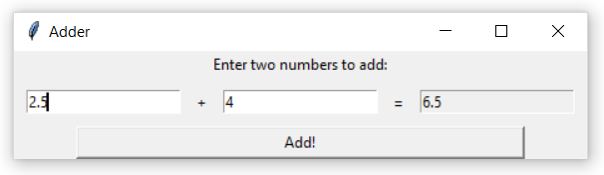
\includegraphics[width=\linewidth,keepaspectratio]{adder}
\end{center}
\end{frame}

%%%%%%%%%%%%%%%%%%%%%%%%%%%%%%%%%%%%%%%%%%%%%%%%%%%
\begin{frame}[fragile] \frametitle{Frames}

\begin{itemize}
\item Container that can be placed within a window
\item Holds other widgets
\item Each frame has its own grid layout, independent of the main window
\item You can use a different layout manager for each container
\end{itemize}
\end{frame}

%%%%%%%%%%%%%%%%%%%%%%%%%%%%%%%%%%%%%%%%%%%%%%%%%%%
\begin{frame}[fragile] \frametitle{Example: Frames (use within GUI class)}
\begin{lstlisting}
f1 = Frame(win, height=100, width=100, bd=1, relief=SUNKEN)
f2 = Frame(win, height=100, width=100, bd=1, relief=SUNKEN)

f1.grid(row=0, column=0, sticky=EW)
f2.grid(row=0, column=1, sticky=EW)

# self.l1 will be used for another method later
self.l1 = Label(f1, text="One", height=5, width=5)
self.l1.grid(row=0, column=0)
Label(f1, text="Two", height=5, width=5).grid(row=0, column=1)
Label(f2, text="Three", height=5, width=5).pack(side=LEFT)
Label(f2, text="Four", height=5, width=5).pack(side=LEFT)

\end{lstlisting}
\end{frame}

%%%%%%%%%%%%%%%%%%%%%%%%%%%%%%%%%%%%%%%%%%%%%%%%%%%
\begin{frame}[fragile] \frametitle{Radiobuttons}
\begin{itemize}
\item Allows the user to choose from one or more options
\item Can be linked to other Radiobuttons with StringVars and IntVars
\item If configured correctly, only one Radiobuttons from a group can be selected at at time
\end{itemize}
\end{frame}

%%%%%%%%%%%%%%%%%%%%%%%%%%%%%%%%%%%%%%%%%%%%%%%%%%%
\begin{frame}[fragile] \frametitle{StringVars and IntVars}
\begin{itemize}
\item Two variable classes included in Tkinter
\item Have .set() method to set their value
e.g. my\_string\_var.set(``Hello'')
\item StringVars have string value, IntVars have integer value
\item Have .get() method to get their value
e.g. val = my\_string\_var.get()
\item Can be passed in as ``variable'' argument when creating a Radiobutton, or ``textvariable'' argument when creating an Entry

\end{itemize}
\end{frame}

%%%%%%%%%%%%%%%%%%%%%%%%%%%%%%%%%%%%%%%%%%%%%%%%%%%
\begin{frame}[fragile] \frametitle{Exercise}
\begin{itemize}
\item Revisit our Adder example from the last class
\item Instead of using Entry.insert and Entry.delete, use a StringVar to change the text of the result Entry
\item See what happens if you don't set the Entry state to ``normal'' before changing the text!
\end{itemize}
\end{frame}

%%%%%%%%%%%%%%%%%%%%%%%%%%%%%%%%%%%%%%%%%%%%%%%%%%%
\begin{frame}[fragile] \frametitle{Adding Radiobuttons to our Frame example}
\begin{lstlisting}
self.color = StringVar()

rb1 = Radiobutton(win, text="Red", variable=self.color, value="red")
rb2 = Radiobutton(win, text="Blue", variable=self.color, value="blue")
rb3 = Radiobutton(win, text="Green", variable=self.color, value="green")

self.color.set("unknown") # deselects all radiobuttons linked to self.color

rb1.grid(row=1, column=0)
rb2.grid(row=2, column=0)
rb3.grid(row=3, column=0)

Button(win, text="Change Color", command=self.change_color).grid(row=1, column=1)
\end{lstlisting}
\end{frame}

%%%%%%%%%%%%%%%%%%%%%%%%%%%%%%%%%%%%%%%%%%%%%%%%%%%
\begin{frame}[fragile] \frametitle{Adding Radiobuttons to our Frame example}

\adjustbox{valign=t}{
\begin{minipage}{0.45\linewidth}
\begin{lstlisting}
def change_color(self):
	new_color = self.color.get()
	if new_color == "unknown":
		pass
       else:
       	self.l1.config(bg=new_color)
\end{lstlisting}
\end{minipage}
}
\hfill
\adjustbox{valign=t}{
\begin{minipage}{0.45\linewidth}
\begin{center}
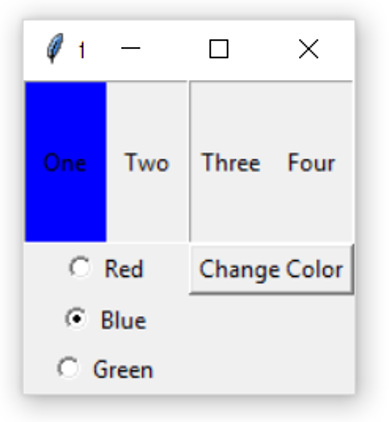
\includegraphics[width=\linewidth,keepaspectratio]{rb1}
\end{center}
\end{minipage}
}
\end{frame}

%%%%%%%%%%%%%%%%%%%%%%%%%%%%%%%%%%%%%%%%%%%%%%%%%%%
\begin{frame}[fragile] \frametitle{Additional Exercise}
\begin{itemize}
\item Add another set of Radiobuttons to the GUI. Separate from those linked to self.change\_color
\item There should be four Radiobuttons, each linked to one of the labels
\item Create an IntVar to use as the variable for these Radiobuttons
\item The user's selection should determine which Label will change color when the button is clicked.
\end{itemize}
\end{frame}

%%%%%%%%%%%%%%%%%%%%%%%%%%%%%%%%%%%%%%%%%%%%%%%%%%%
\begin{frame}[fragile] \frametitle{Root Window vs. Toplevels}
\begin{itemize}
\item The root window is your main window (Tk)
\item A GUI application should have only one root window
\item Any additional windows should be Toplevels
\item Hide windows with .withdraw()
\item Show windows with .deiconify()
\item Delete windows with .destroy() (they will be gone forever!)
\item If you destroy the root window, all Toplevels will also be destroyed

\end{itemize}
\end{frame}

%%%%%%%%%%%%%%%%%%%%%%%%%%%%%%%%%%%%%%%%%%%%%%%%%%%
\begin{frame}[fragile] \frametitle{Adding multiple windows to our example}
\begin{lstlisting}
# in __init__ method, add line: self.root = win

def new_window(self):
	self.root.withdraw()
	self.new = Toplevel()
	Label(self.new, width=30, height=10, text="I'm a new window!").pack()
	Button(self.new, text="Close window", command=self.close_new).pack()

def close_new(self):
	self.new.destroy() # destroy new window
	self.root.deiconify() # show root window

\end{lstlisting}
\end{frame}


%%%%%%%%%%%%%%%%%%%%%%%%%%%%%%%%%%%%%%%%%%%%%%%%%%%
\begin{frame}[fragile] \frametitle{Changing the GUI appearance}
\begin{itemize}
\item GUI windows and widgets have many optional parameters to change their appearance
\item bg: background color
\item fg: foreground color (for Labels, this is the font color)
\item bd: border width
\item border: border type (RAISED, SUNKEN, etc)
\item For color codes: http://htmlcolorcodes.com/ 
\item For more options, check the documentation or online tutorials
\end{itemize}
\end{frame}






%%
%%
%%%%%%%%%%%%%%%%%%%%%%%%%%%%%%%%%%%%%%%%%%%%%%%%%%%%%%%%%%%%%%%%%%%%%%%%%%%%%%%%%%%%
%%\begin{frame}[fragile]\frametitle{Graphical User Interfaces with Tkinter}
%%
%%Tk/Tcl has long been an integral part of Python.  It provides a robust
%%and platform independent windowing toolkit, that is available to
%%Python programmers using the \textbf{Tkinter} module, and its
%%extension, the \textbf{Tix} module.
%%
%%The \textbf{Tkinter} module is a thin object--oriented layer on top of
%%Tcl/Tk. To use \textbf{Tkinter}, you don't need to write Tcl code,
%%but you will need to consult the Tk documentation, and occasionally
%%the Tcl documentation.  \textbf{Tkinter} is a set of wrappers that
%%implement the Tk widgets as Python classes.  In addition, the internal
%%module \textbf{\_tkinter} provides a threadsafe mechanism which allows
%%Python and Tcl to interact.
%%
%%Tk is not the only GUI for Python, but is however the most commonly
%%used one; see section~\ref{other-gui-modules}, ``Other User Interface
%%Modules and Packages,'' for more information on other GUI toolkits for
%%Python.
%%\end{frame}
%%
%%
%%%%%%%%%%%%%%%%%%%%%%%%%%%%%%%%%%%%%%%%%%%%%%%%%%%%%%%%%%%%%%%%%%%%%%%%%%%%%%%%%%%%
%%\begin{frame}[fragile]\frametitle{Tkinter: Python interface to Tcl/Tk}
%%
%%The Tkinter module (``Tk interface'') is the standard Python
%%interface to the Tk GUI toolkit.  Both Tk and Tkinter are
%%available on most UNIX platforms, as well as on Windows and
%%Macintosh systems.  (Tk itself is not part of Python; it is maintained
%%at ActiveState.)
%%
%%\end{frame}
%%
%%
%%%%%%%%%%%%%%%%%%%%%%%%%%%%%%%%%%%%%%%%%%%%%%%%%%%%%%%%%%%%%%%%%%%%%%%%%%%%%%%%%%%%
%%\begin{frame}[fragile]\frametitle{Tkinter Modules}
%%
%%Most of the time, the \textbf{Tkinter} module is all you really
%%need, but a number of additional modules are available as well.  The
%%Tk interface is located in a binary module named \textbf{\_tkinter}.
%%This module contains the low-level interface to Tk, and should never
%%be used directly by application programmers. It is usually a shared
%%library (or DLL), but might in some cases be statically linked with
%%the Python interpreter.
%%
%%In addition to the Tk interface module, \textbf{Tkinter} includes a
%%number of Python modules. The two most important modules are the
%%\textbf{Tkinter} module itself, and a module called
%%\textbf{Tkconstants}. The former automatically imports the latter, so
%%to use Tkinter, all you need to do is to import one module:
%%
%%\begin{lstlisting}
%%import Tkinter
%%\end{lstlisting}
%%
%%Or, more often:
%%
%%\begin{lstlisting}
%%from Tkinter import *
%%\end{lstlisting}
%%
%%\end{frame}
%%
%%%%%%%%%%%%%%%%%%%%%%%%%%%%%%%%%%%%%%%%%%%%%%%%%%%%%%%%%%%%%%%%%%%%%%%%%%%%%%%%%%%%
%%\begin{frame}[fragile]\frametitle{Tkinter Modules}
%%
%%
%%The \textbf{Tk} class is instantiated without arguments.
%%This creates a toplevel widget of Tk which usually is the main window
%%of an appliation. Each instance has its own associated Tcl interpreter.
%%% FIXME: The following keyword arguments are currently recognized:
%%
%%Other modules that provide Tk support include:
%%
%%\begin{itemize}
%%% \declaremodule{standard}{Tkconstants}
%%% \modulesynopsis{Constants used by Tkinter}
%%% FIXME 
%%
%%\item[\textbf{ScrolledText}]
%%Text widget with a vertical scroll bar built in.
%%
%%\item[\textbf{tkColorChooser}]
%%Dialog to let the user choose a color.
%%
%%\item[\textbf{tkCommonDialog}]
%%Base class for the dialogs defined in the other modules listed here.
%%
%%\item[\textbf{tkFileDialog}]
%%Common dialogs to allow the user to specify a file to open or save.
%%
%%\item[\textbf{tkFont}]
%%Utilities to help work with fonts.
%%
%%\item[\textbf{tkMessageBox}]
%%Access to standard Tk dialog boxes.
%%
%%\item[\textbf{tkSimpleDialog}]
%%Basic dialogs and convenience functions.
%%
%%\item[\textbf{Tkdnd}]
%%Drag-and-drop support for \textbf{Tkinter}.
%%This is experimental and should become deprecated when it is replaced 
%%with the Tk DND.
%%
%%\item[\textbf{turtle}]
%%Turtle graphics in a Tk window.
%%
%%\end{itemize}
%%\end{frame}
%%
%%
%%%%%%%%%%%%%%%%%%%%%%%%%%%%%%%%%%%%%%%%%%%%%%%%%%%%%%%%%%%%%%%%%%%%%%%%%%%%%%%%%%%%
%%\begin{frame}[fragile]\frametitle{Tkinter Life Preserver}
%%
%%% Converted to LaTeX by Mike Clarkson.
%%
%%This section is not designed to be an exhaustive tutorial on either
%%Tk or Tkinter.  Rather, it is intended as a stop gap, providing some
%%introductory orientation on the system.
%%
%%Credits:
%%\begin{itemize}
%%\item   Tkinter was written by Steen Lumholt and Guido van Rossum.
%%\item   Tk was written by John Ousterhout while at Berkeley.
%%\item   This Life Preserver was written by Matt Conway at
%%the University of Virginia.
%%\item   The html rendering, and some liberal editing, was
%%produced from a FrameMaker version by Ken Manheimer.
%%\item   Fredrik Lundh elaborated and revised the class interface descriptions,
%%to get them current with Tk 4.2.
%%\item  Mike Clarkson converted the documentation to \LaTeX, and compiled the 
%%User Interface chapter of the reference manual.
%%\end{itemize}
%%\end{frame}
%%
%%
%%%%%%%%%%%%%%%%%%%%%%%%%%%%%%%%%%%%%%%%%%%%%%%%%%%%%%%%%%%%%%%%%%%%%%%%%%%%%%%%%%%%
%%\begin{frame}[fragile]\frametitle{How To Use This Section}
%%
%%This section is designed in two parts: the first half (roughly) covers
%%background material, while the second half can be taken to the
%%keyboard as a handy reference.
%%
%%When trying to answer questions of the form ``how do I do blah'', it
%%is often best to find out how to do``blah'' in straight Tk, and then
%%convert this back into the corresponding \textbf{Tkinter} call.
%%Python programmers can often guess at the correct Python command by
%%looking at the Tk documentation. This means that in order to use
%%Tkinter, you will have to know a little bit about Tk. This document
%%can't fulfill that role, so the best we can do is point you to the
%%best documentation that exists. Here are some hints:
%%
%%\begin{itemize}
%%\item   The authors strongly suggest getting a copy of the Tk man
%%pages. Specifically, the man pages in the \code{mann} directory are most
%%useful. The \code{man3} man pages describe the C interface to the Tk
%%library and thus are not especially helpful for script writers.  
%%
%%\item   Addison-Wesley publishes a book called \textbf{Tcl and the
%%Tk Toolkit} by John Ousterhout (ISBN 0-201-63337-X) which is a good
%%introduction to Tcl and Tk for the novice.  The book is not
%%exhaustive, and for many details it defers to the man pages. 
%%
%%\item   \textbf{Tkinter.py} is a last resort for most, but can be a good
%%place to go when nothing else makes sense.  
%%\end{itemize}
%%
%%\end{frame}
%%
%%
%%%%%%%%%%%%%%%%%%%%%%%%%%%%%%%%%%%%%%%%%%%%%%%%%%%%%%%%%%%%%%%%%%%%%%%%%%%%%%%%%%%%
%%\begin{frame}[fragile]\frametitle{A Simple Hello World Program} % HelloWorld.html
%%
%%%begin{latexonly}
%%%\begin{figure}[hbtp]
%%%\centerline{\epsfig{file=HelloWorld.gif,width=.9\textwidth}}
%%%\vspace{.5cm}
%%%\caption{HelloWorld gadget image}
%%%\end{figure}
%%%See also the hello-world \ulink{notes}{classes/HelloWorld-notes.html} and
%%%\ulink{summary}{classes/HelloWorld-summary.html}.
%%%end{latexonly}
%%
%%
%%\begin{lstlisting}
%%from Tkinter import *                                                    1
%%                                                                         2
%%class Application(Frame):                                                3
%%    def say_hi(self):                                                    4
%%        print ''hi there, everyone!''                                      5
%%                                                                         6
%%    def createWidgets(self):                                             7
%%        self.QUIT = Button(self)                                         8
%%        self.QUIT[''text''] = ''QUIT''                                       9
%%        self.QUIT[''fg'']   = ''red''                                       10
%%        self.QUIT[''command''] =  self.quit                               11
%%                                                                        12
%%        self.QUIT.pack({''side'': ''left''})                                13
%%                                                                        14
%%        self.hi_there = Button(self)                                    15
%%        self.hi_there[''text''] = ''Hello'',                                16
%%        self.hi_there[''command''] = self.say_hi                          17
%%                                                                        18
%%        self.hi_there.pack({''side'': ''left''})                            19
%%                                                                        20
%%                                                                        21
%%    def __init__(self, master=None):                                    22
%%        Frame.__init__(self, master)                                    23
%%        self.pack()                                                     24
%%        self.createWidgets()                                            25
%%                                                                        26
%%app = Application()                                                     27
%%app.mainloop()                                                          28
%%\end{lstlisting}
%%\end{frame}
%%
%%%%%%%%%%%%%%%%%%%%%%%%%%%%%%%%%%%%%%%%%%%%%%%%%%%%%%%%%%%%%%%%%%%%%%%%%%%%%%%%%%%%
%%\begin{frame}[fragile]\frametitle{A (Very) Quick Look at Tcl/Tk} % BriefTclTk.html
%%
%%The class hierarchy looks complicated, but in actual practice,
%%application programmers almost always refer to the classes at the very
%%bottom of the hierarchy. 
%%
%%Notes:
%%\begin{itemize}
%%\item   These classes are provided for the purposes of
%%organizing certain functions under one namespace. They aren't meant to
%%be instantiated independently.
%%
%%\item    The \textbf{Tk} class is meant to be instantiated only once in
%%an application. Application programmers need not instantiate one
%%explicitly, the system creates one whenever any of the other classes
%%are instantiated.
%%
%%\item    The \textbf{Widget} class is not meant to be instantiated, it
%%is meant only for subclassing to make ``real'' widgets (in Cpp, this
%%is called an `abstract class').
%%\end{itemize}
%%
%%To make use of this reference material, there will be times when you
%%will need to know how to read short passages of Tk and how to identify
%%the various parts of a Tk command.  
%%(See section~\ref{tkinter-basic-mapping} for the
%%\textbf{Tkinter} equivalents of what's below.)
%%
%%\end{frame}
%%
%%%%%%%%%%%%%%%%%%%%%%%%%%%%%%%%%%%%%%%%%%%%%%%%%%%%%%%%%%%%%%%%%%%%%%%%%%%%%%%%%%%%
%%\begin{frame}[fragile]\frametitle{A (Very) Quick Look at Tcl/Tk} % BriefTclTk.html
%%
%%Tk scripts are Tcl programs.  Like all Tcl programs, Tk scripts are
%%just lists of tokens separated by spaces.  A Tk widget is just its
%%\emph{class}, the \emph{options} that help configure it, and the
%%\emph{actions} that make it do useful things. 
%%
%%To make a widget in Tk, the command is always of the form: 
%%
%%\begin{lstlisting}
%%                classCommand newPathname options
%%\end{lstlisting}
%%
%%\begin{itemize}
%%\item[\textbf{classCommand}]
%%denotes which kind of widget to make (a button, a label, a menu...)
%%
%%\item[\textbf{newPathname}]
%%is the new name for this widget.  All names in Tk must be unique.  To
%%help enforce this, widgets in Tk are named with \emph{pathnames}, just
%%like files in a file system.  The top level widget, the \emph{root},
%%is called \code{.} (period) and children are delimited by more
%%periods.  For example, \code{.myApp.controlPanel.okButton} might be
%%the name of a widget.
%%
%%\item[\textbf{options} ]
%%configure the widget's appearance and in some cases, its
%%behavior.  The options come in the form of a list of flags and values.
%%Flags are proceeded by a `-', like unix shell command flags, and
%%values are put in quotes if they are more than one word.
%%\end{itemize}
%%
%%\end{frame}
%%
%%%%%%%%%%%%%%%%%%%%%%%%%%%%%%%%%%%%%%%%%%%%%%%%%%%%%%%%%%%%%%%%%%%%%%%%%%%%%%%%%%%%
%%\begin{frame}[fragile]\frametitle{A (Very) Quick Look at Tcl/Tk} % BriefTclTk.html
%%
%%For example: 
%%
%%\begin{lstlisting}
%%    button   .fred   -fg red -text ''hi there''
%%       ^       ^     \_____________________/
%%       |       |                |
%%     class    new            options
%%    command  widget  (-opt val -opt val ...)
%%\end{lstlisting} 
%%
%%Once created, the pathname to the widget becomes a new command.  This
%%new \textbf{widget command} is the programmer's handle for getting the new
%%widget to perform some \textbf{action}.  In C, you'd express this as
%%someAction(fred, someOptions), in Cpp, you would express this as
%%fred.someAction(someOptions), and in Tk, you say: 
%%
%%\begin{lstlisting}
%%    .fred someAction someOptions 
%%\end{lstlisting} 
%%
%%Note that the object name, \code{.fred}, starts with a dot.
%%
%%As you'd expect, the legal values for \textbf{someAction} will depend on
%%the widget's class: \code{.fred disable} works if fred is a
%%button (fred gets greyed out), but does not work if fred is a label
%%(disabling of labels is not supported in Tk). 
%%
%%The legal values of \textbf{someOptions} is action dependent.  Some
%%actions, like \code{disable}, require no arguments, others, like
%%a text-entry box's \code{delete} command, would need arguments
%%to specify what range of text to delete.  
%%\end{frame}
%%
%%
%%%%%%%%%%%%%%%%%%%%%%%%%%%%%%%%%%%%%%%%%%%%%%%%%%%%%%%%%%%%%%%%%%%%%%%%%%%%%%%%%%%%
%%\begin{frame}[fragile]\frametitle{Mapping Basic Tk into Tkinter} % BriefTclTk.html
%%
%%
%%Class commands in Tk correspond to class constructors in Tkinter.
%%
%%\begin{lstlisting}
%%    button .fred                =====>  fred = Button()
%%\end{lstlisting}
%%
%%The master of an object is implicit in the new name given to it at
%%creation time.  In Tkinter, masters are specified explicitly.
%%
%%\begin{lstlisting}
%%    button .panel.fred          =====>  fred = Button(panel)
%%\end{lstlisting}
%%
%%The configuration options in Tk are given in lists of hyphened tags
%%followed by values.  In Tkinter, options are specified as
%%keyword-arguments in the instance constructor, and keyword-args for
%%configure calls or as instance indices, in dictionary style, for
%%established instances.  See section~\ref{tkinter-setting-options} on
%%setting options.
%%
%%\begin{lstlisting}
%%    button .fred -fg red        =====>  fred = Button(panel, fg = ''red'')
%%    .fred configure -fg red     =====>  fred[''fg''] = red
%%                                OR ==>  fred.config(fg = ''red'')
%%\end{lstlisting}
%%
%%\end{frame}
%%
%%%%%%%%%%%%%%%%%%%%%%%%%%%%%%%%%%%%%%%%%%%%%%%%%%%%%%%%%%%%%%%%%%%%%%%%%%%%%%%%%%%%
%%\begin{frame}[fragile]\frametitle{} % BriefTclTk.html
%%In Tk, to perform an action on a widget, use the widget name as a
%%command, and follow it with an action name, possibly with arguments
%%(options).  In Tkinter, you call methods on the class instance to
%%invoke actions on the widget.  The actions (methods) that a given
%%widget can perform are listed in the Tkinter.py module.
%%
%%\begin{lstlisting}
%%    .fred invoke                =====>  fred.invoke()
%%\end{lstlisting}
%%
%%To give a widget to the packer (geometry manager), you call pack with
%%optional arguments.  In Tkinter, the Pack class holds all this
%%functionality, and the various forms of the pack command are
%%implemented as methods.  All widgets in \textbf{Tkinter} are
%%subclassed from the Packer, and so inherit all the packing
%%methods. See the \textbf{Tix} module documentation for additional
%%information on the Form geometry manager.
%%
%%\begin{lstlisting}
%%    pack .fred -side left       =====>  fred.pack(side = ''left'')
%%\end{lstlisting}
%%\end{frame}
%%
%%
%%%%%%%%%%%%%%%%%%%%%%%%%%%%%%%%%%%%%%%%%%%%%%%%%%%%%%%%%%%%%%%%%%%%%%%%%%%%%%%%%%%%
%%\begin{frame}[fragile]\frametitle{How Tk and Tkinter are Related} % Relationship.html
%%
%%\note{This was derived from a graphical image; the image will be used
%%      more directly in a subsequent version of this document.}
%%
%%From the top down:
%%\begin{itemize}
%%\item[\textbf{Your App Here (Python)}]
%%A Python application makes a \textbf{Tkinter} call.
%%
%%\item[\textbf{Tkinter (Python Module)}]
%%This call (say, for example, creating a button widget), is
%%implemented in the \emph{Tkinter} module, which is written in
%%Python.  This Python function will parse the commands and the
%%arguments and convert them into a form that makes them look as if they
%%had come from a Tk script instead of a Python script.
%%
%%\item[\textbf{tkinter (C)}]
%%These commands and their arguments will be passed to a C function
%%in the \emph{tkinter} - note the lowercase - extension module.
%%
%%\item[\textbf{Tk Widgets} (C and Tcl)]
%%This C function is able to make calls into other C modules,
%%including the C functions that make up the Tk library.  Tk is
%%implemented in C and some Tcl.  The Tcl part of the Tk widgets is used
%%to bind certain default behaviors to widgets, and is executed once at
%%the point where the Python \textbf{Tkinter} module is
%%imported. (The user never sees this stage).
%%
%%\item[\textbf{Tk (C)}]
%%The Tk part of the Tk Widgets implement the final mapping to ...
%%
%%\item[\textbf{Xlib (C)}]
%%the Xlib library to draw graphics on the screen.
%%\end{itemize}
%%
%%\end{frame}
%%
%%
%%%%%%%%%%%%%%%%%%%%%%%%%%%%%%%%%%%%%%%%%%%%%%%%%%%%%%%%%%%%%%%%%%%%%%%%%%%%%%%%%%%%
%%\begin{frame}[fragile]\frametitle{Setting Options -tkinter-setting-options}
%%
%%Options control things like the color and border width of a widget.
%%Options can be set in three ways:
%%
%%\begin{itemize}
%%\item[At object creation time, using keyword arguments]:
%%\begin{lstlisting}
%%fred = Button(self, fg = ''red'', bg = ''blue'')
%%\end{lstlisting}
%%\item[After object creation, treating the option name like a dictionary index]:
%%\begin{lstlisting}
%%fred[''fg''] = ''red''
%%fred[''bg''] = ''blue''
%%\end{lstlisting}
%%\item[Use the config() method to update multiple attrs subesequent to
%%object creation]:
%%\begin{lstlisting}
%%fred.config(fg = ''red'', bg = ''blue'')
%%\end{lstlisting}
%%\end{itemize}
%%
%%\end{frame}
%%
%%%%%%%%%%%%%%%%%%%%%%%%%%%%%%%%%%%%%%%%%%%%%%%%%%%%%%%%%%%%%%%%%%%%%%%%%%%%%%%%%%%%
%%\begin{frame}[fragile]\frametitle{Setting Options -tkinter-setting-options}
%%
%%For a complete explanation of a given option and its behavior, see the
%%Tk man pages for the widget in question.
%%
%%Note that the man pages list ''STANDARD OPTIONS'' and ''WIDGET SPECIFIC
%%OPTIONS'' for each widget.  The former is a list of options that are
%%common to many widgets, the latter are the options that are
%%ideosyncratic to that particular widget. 
%%No distinction between standard and widget-specific options is made in
%%this document.  Some options don't apply to some kinds of widgets.
%%Whether a given widget responds to a particular option depends on the
%%class of the widget; buttons have a \code{command} option, labels do not. 
%%
%%The options supported by a given widget are listed in that widget's
%%man page, or can be queried at runtime by calling the
%%\textbf{config()} method without arguments, or by calling the
%%\textbf{keys()} method on that widget.  The return value of these
%%calls is a dictionary whose key is the name of the option as a string
%%(for example, \code{'relief'}) and whose values are 5-tuples.
%%
%%\end{frame}
%%
%%%%%%%%%%%%%%%%%%%%%%%%%%%%%%%%%%%%%%%%%%%%%%%%%%%%%%%%%%%%%%%%%%%%%%%%%%%%%%%%%%%%
%%\begin{frame}[fragile]\frametitle{Setting Options -tkinter-setting-options}
%%Some options, like \code{bg} are synonyms for common options with long
%%names (\code{bg} is shorthand for ''background''). Passing the
%%\code{config()} method the name of a shorthand option will return a
%%2-tuple, not 5-tuple. The 2-tuple passed back will contain the name of
%%the synonym and the ``real'' option (such as \code{('bg',
%%'background')}).
%%
%%%\begin{table}{c|l|l}{textrm}{Index}{Meaning}{Example}
%%%  \lineiii{0}{option name}                       {\code{'relief'}}
%%%  \lineiii{1}{option name for database lookup}   {\code{'relief'}}
%%%  \lineiii{2}{option class for database lookup}  {\code{'Relief'}}
%%%  \lineiii{3}{default value}                     {\code{'raised'}}
%%%  \lineiii{4}{current value}                     {\code{'groove'}}
%%%\end{table}
%%
%%
%%Example:
%%
%%\begin{lstlisting}
%%>>> print fred.config()
%%{'relief' : ('relief', 'relief', 'Relief', 'raised', 'groove')}
%%\end{lstlisting}
%%
%%Of course, the dictionary printed will include all the options
%%available and their values.  This is meant only as an example.
%%
%%\end{frame}
%%
%%
%%
%%%%%%%%%%%%%%%%%%%%%%%%%%%%%%%%%%%%%%%%%%%%%%%%%%%%%%%%%%%%%%%%%%%%%%%%%%%%%%%%%%%%
%%\begin{frame}[fragile]\frametitle{The Packer} % Packer.html
%%
%%
%%The packer is one of Tk's geometry-management mechanisms.  See also
%%\textbf[classes/ClassPacker.html]{the Packer class interface}.
%%
%%Geometry managers are used to specify the relative positioning of the
%%positioning of widgets within their container - their mutual
%%\emph{master}.  In contrast to the more cumbersome \emph{placer}
%%(which is used less commonly, and we do not cover here), the packer
%%takes qualitative relationship specification - \emph{above}, \emph{to
%%the left of}, \emph{filling}, etc - and works everything out to
%%determine the exact placement coordinates for you. 
%%
%%The size of any \emph{master} widget is determined by the size of
%%the ''slave widgets'' inside.  The packer is used to control where slave
%%widgets appear inside the master into which they are packed.  You can
%%pack widgets into frames, and frames into other frames, in order to
%%achieve the kind of layout you desire.  Additionally, the arrangement
%%is dynamically adjusted to accomodate incremental changes to the
%%configuration, once it is packed.
%%
%%Note that widgets do not appear until they have had their geometry
%%specified with a geometry manager.  It's a common early mistake to
%%leave out the geometry specification, and then be surprised when the
%%widget is created but nothing appears.  A widget will appear only
%%after it has had, for example, the packer's \textbf{pack()} method
%%applied to it.
%%
%%The pack() method can be called with keyword-option/value pairs that
%%control where the widget is to appear within its container, and how it
%%is to behave when the main application window is resized.  Here are
%%some examples:
%%
%%\begin{lstlisting}
%%    fred.pack()                     # defaults to side = ''top''
%%    fred.pack(side = ''left'')
%%    fred.pack(expand = 1)
%%\end{lstlisting}
%%
%%\end{frame}
%%
%%
%%%%%%%%%%%%%%%%%%%%%%%%%%%%%%%%%%%%%%%%%%%%%%%%%%%%%%%%%%%%%%%%%%%%%%%%%%%%%%%%%%%%
%%\begin{frame}[fragile]\frametitle{Packer Options}
%%
%%For more extensive information on the packer and the options that it
%%can take, see the man pages and page 183 of John Ousterhout's book.
%%
%%\begin{itemize}
%%\item[\textbf{anchor }]
%%Anchor type.  Denotes where the packer is to place each slave in its
%%parcel.
%%
%%\item[\textbf{expand}]
%%Boolean, \code{0} or \code{1}.
%%
%%\item[\textbf{fill}]
%%Legal values: \code{'x'}, \code{'y'}, \code{'both'}, \code{'none'}.
%%
%%\item[\textbf{ipadx} and \textbf{ipady}]
%%A distance - designating internal padding on each side of the slave
%%widget.
%%
%%\item[\textbf{padx} and \textbf{pady}]
%%A distance - designating external padding on each side of the slave
%%widget.
%%
%%\item[\textbf{side}]
%%Legal values are: \code{'left'}, \code{'right'}, \code{'top'},
%%\code{'bottom'}.
%%\end{itemize}
%%
%%\end{frame}
%%

%%\subsubsection{Coupling Widget Variables} % VarCouplings.html
%%
%%The current-value setting of some widgets (like text entry widgets)
%%can be connected directly to application variables by using special
%%options.  These options are \code{variable}, \code{textvariable},
%%\code{onvalue}, \code{offvalue}, and \code{value}.  This
%%connection works both ways: if the variable changes for any reason,
%%the widget it's connected to will be updated to reflect the new value. 
%%
%%Unfortunately, in the current implementation of \textbf{Tkinter} it is
%%not possible to hand over an arbitrary Python variable to a widget
%%through a \code{variable} or \code{textvariable} option.  The only
%%kinds of variables for which this works are variables that are
%%subclassed from a class called Variable, defined in the
%%\textbf{Tkinter} module.
%%
%%There are many useful subclasses of Variable already defined:
%%\textbf{StringVar}, \textbf{IntVar}, \textbf{DoubleVar}, and
%%\textbf{BooleanVar}.  To read the current value of such a variable,
%%call the \textbf{get()} method on
%%it, and to change its value you call the \textbf{set()} method.  If
%%you follow this protocol, the widget will always track the value of
%%the variable, with no further intervention on your part.
%%
%%For example: 
%%\begin{lstlisting}
%%class App(Frame):
%%    def __init__(self, master=None):
%%        Frame.__init__(self, master)
%%        self.pack()
%%        
%%        self.entrythingy = Entry()
%%        self.entrythingy.pack()
%%        
%%        self.button.pack()
%%        # here is the application variable
%%        self.contents = StringVar()
%%        # set it to some value
%%        self.contents.set(''this is a variable'')
%%        # tell the entry widget to watch this variable
%%        self.entrythingy[''textvariable''] = self.contents
%%        
%%        # and here we get a callback when the user hits return.
%%        # we will have the program print out the value of the
%%        # application variable when the user hits return
%%        self.entrythingy.bind('<Key-Return>',
%%                              self.print_contents)
%%
%%    def print_contents(self, event):
%%        print ''hi. contents of entry is now ---->'', \
%%              self.contents.get()
%%\end{lstlisting}
%%
%%
%%\subsubsection{The Window Manager} % WindowMgr.html
%%\index{window manager (widgets)}
%%
%%In Tk, there is a utility command, \code{wm}, for interacting with the
%%window manager.  Options to the \code{wm} command allow you to control
%%things like titles, placement, icon bitmaps, and the like.  In
%%\textbf{Tkinter}, these commands have been implemented as methods
%%on the \textbf{Wm} class.  Toplevel widgets are subclassed from the
%%\textbf{Wm} class, and so can call the \textbf{Wm} methods directly.
%%
%%%See also \textbf[classes/ClassWm.html]{the Wm class interface}.
%%
%%To get at the toplevel window that contains a given widget, you can
%%often just refer to the widget's master.  Of course if the widget has
%%been packed inside of a frame, the master won't represent a toplevel
%%window.  To get at the toplevel window that contains an arbitrary
%%widget, you can call the \textbf{_root()} method.  This
%%method begins with an underscore to denote the fact that this function
%%is part of the implementation, and not an interface to Tk functionality.
%%
%%Here are some examples of typical usage:
%%
%%\begin{lstlisting}
%%import Tkinter
%%class App(Frame):
%%    def __init__(self, master=None):
%%        Frame.__init__(self, master)
%%        self.pack()
%%
%%
%%# create the application
%%myapp = App()
%%
%%#
%%# here are method calls to the window manager class
%%#
%%myapp.master.title(''My Do-Nothing Application'')
%%myapp.master.maxsize(1000, 400)
%%
%%# start the program
%%myapp.mainloop()
%%\end{lstlisting}
%%
%%
%%\subsubsection{Tk Option Data Types} % OptionTypes.html
%%
%%\index{Tk Option Data Types}
%%
%%\begin{itemize}
%%\item[anchor]
%%Legal values are points of the compass: \code{''n''},
%%\code{''ne''}, \code{''e''}, \code{''se''}, \code{''s''},
%%\code{''sw''}, \code{''w''}, \code{''nw''}, and also
%%\code{''center''}.
%%
%%\item[bitmap]
%%There are eight built-in, named bitmaps: \code{'error'}, \code{'gray25'},
%%\code{'gray50'}, \code{'hourglass'}, \code{'info'}, \code{'questhead'},
%%\code{'question'}, \code{'warning'}.  To specify an X bitmap
%%filename, give the full path to the file, preceded with an \code{@},
%%as in \code{''@/usr/contrib/bitmap/gumby.bit''}.
%%
%%\item[boolean]
%%You can pass integers 0 or 1 or the stings \code{''yes''} or \code{''no''} .
%%
%%\item[callback]
%%This is any Python function that takes no arguments.  For example: 
%%\begin{lstlisting}
%%    def print_it():
%%            print ''hi there''
%%    fred[''command''] = print_it
%%\end{lstlisting}
%%
%%\item[color]
%%Colors can be given as the names of X colors in the rgb.txt file,
%%or as strings representing RGB values in 4 bit: \code{''\#RGB''}, 8
%%bit: \code{''\#RRGGBB''}, 12 bit'' \code{''\#RRRGGGBBB''}, or 16 bit
%%\code{''\#RRRRGGGGBBBB''} ranges, where R,G,B here represent any
%%legal hex digit.  See page 160 of Ousterhout's book for details.  
%%
%%\item[cursor]
%%The standard X cursor names from \textbf{cursorfont.h} can be used,
%%without the \code{XC_} prefix.  For example to get a hand cursor
%%(\constant{XC_hand2}), use the string \code{''hand2''}.  You can also
%%specify a bitmap and mask file of your own.  See page 179 of
%%Ousterhout's book.
%%
%%\item[distance]
%%Screen distances can be specified in either pixels or absolute
%%distances.  Pixels are given as numbers and absolute distances as
%%strings, with the trailing character denoting units: \code{c}
%%for centimeters, \code{i} for inches, \code{m} for millimeters,
%%\code{p} for printer's points.  For example, 3.5 inches is expressed
%%as \code{''3.5i''}.
%%
%%\item[font]
%%Tk uses a list font name format, such as \code{\{courier 10 bold\}}.
%%Font sizes with positive numbers are measured in points;
%%sizes with negative numbers are measured in pixels.
%%
%%\item[geometry]
%%This is a string of the form \samp{\textbf{width}x\textbf{height}}, where
%%width and height are measured in pixels for most widgets (in
%%characters for widgets displaying text).  For example:
%%\code{fred[''geometry''] = ''200x100''}.
%%
%%\item[justify]
%%Legal values are the strings: \code{''left''},
%%\code{''center''}, \code{''right''}, and \code{''fill''}.
%%
%%\item[region]
%%This is a string with four space-delimited elements, each of
%%which is a legal distance (see above).  For example: \code{''2 3 4
%%5''} and \code{''3i 2i 4.5i 2i''} and \code{''3c 2c 4c 10.43c''} 
%%are all legal regions.
%%
%%\item[relief]
%%Determines what the border style of a widget will be.  Legal
%%values are: \code{''raised''}, \code{''sunken''},
%%\code{''flat''}, \code{''groove''}, and \code{''ridge''}.
%%
%%\item[scrollcommand]
%%This is almost always the \textbf{set()} method of some scrollbar
%%widget, but can be any widget method that takes a single argument.  
%%Refer to the file \textbf{Demo/tkinter/matt/canvas-with-scrollbars.py}
%%in the Python source distribution for an example.
%%
%%\item[wrap:]
%%Must be one of: \code{''none''}, \code{''char''}, or \code{''word''}.
%%\end{itemize}
%%
%%
%%\subsubsection{Bindings and Events} % Bindings.html
%%
%%\index{bind (widgets)}
%%\index{events (widgets)}
%%
%%The bind method from the widget command allows you to watch for
%%certain events and to have a callback function trigger when that event
%%type occurs.  The form of the bind method is:
%%
%%\begin{lstlisting}
%%    def bind(self, sequence, func, add=''):
%%\end{lstlisting}
%%where:
%%
%%\begin{itemize}
%%\item[sequence]
%%is a string that denotes the target kind of event.  (See the bind
%%man page and page 201 of John Ousterhout's book for details).
%%
%%\item[func]
%%is a Python function, taking one argument, to be invoked when the
%%event occurs.  An Event instance will be passed as the argument.
%%(Functions deployed this way are commonly known as \textbf{callbacks}.)
%%
%%\item[add]
%%is optional, either \samp{} or \samp{+}.  Passing an empty string
%%denotes that this binding is to replace any other bindings that this
%%event is associated with.  Preceeding with a \samp{+} means that this
%%function is to be added to the list of functions bound to this event type.
%%\end{itemize}
%%
%%For example:
%%\begin{lstlisting}
%%    def turnRed(self, event):
%%        event.widget[''activeforeground''] = ''red''
%%
%%    self.button.bind(''<Enter>'', self.turnRed)
%%\end{lstlisting}
%%
%%Notice how the widget field of the event is being accesed in the
%%\textbf{turnRed()} callback.  This field contains the widget that
%%caught the X event.  The following table lists the other event fields
%%you can access, and how they are denoted in Tk, which can be useful
%%when referring to the Tk man pages.
%%
%%\begin{lstlisting}
%%Tk      Tkinter Event Field             Tk      Tkinter Event Field 
%%--      -------------------             --      -------------------
%%%f      focus                           %A      char
%%%h      height                          %E      send_event
%%%k      keycode                         %K      keysym
%%%s      state                           %N      keysym_num
%%%t      time                            %T      type
%%%w      width                           %W      widget
%%%x      x                               %X      x_root
%%%y      y                               %Y      y_root
%%\end{lstlisting}
%%
%%
%%\subsubsection{The index Parameter} % Index.html
%%
%%A number of widgets require``index'' parameters to be passed.  These
%%are used to point at a specific place in a Text widget, or to
%%particular characters in an Entry widget, or to particular menu items
%%in a Menu widget.
%%
%%\begin{itemize}
%%\item[\textbf{Entry widget indexes (index, view index, etc.)}]
%%Entry widgets have options that refer to character positions in the
%%text being displayed.  You can use these \textbf{Tkinter} functions
%%to access these special points in text widgets:
%%
%%\begin{itemize}
%%\item[AtEnd()]
%%refers to the last position in the text
%%
%%\item[AtInsert()]
%%refers to the point where the text cursor is
%%
%%\item[AtSelFirst()]
%%indicates the beginning point of the selected text
%%
%%\item[AtSelLast()]
%%denotes the last point of the selected text and finally
%%
%%\item[At(x\optional{, y})]
%%refers to the character at pixel location \textbf{x}, \textbf{y} (with
%%\textbf{y} not used in the case of a text entry widget, which contains a
%%single line of text).
%%\end{itemize}
%%
%%\item[\textbf{Text widget indexes}]
%%The index notation for Text widgets is very rich and is best described
%%in the Tk man pages.
%%
%%\item[\textbf{Menu indexes (menu.invoke(), menu.entryconfig(), etc.)}]
%%
%%Some options and methods for menus manipulate specific menu entries.
%%Anytime a menu index is needed for an option or a parameter, you may
%%pass in: 
%%\begin{itemize}
%%\item   an integer which refers to the numeric position of the entry in
%%the widget, counted from the top, starting with 0; 
%%\item   the string \code{'active'}, which refers to the menu position that is
%%currently under the cursor;
%%\item   the string \code{''last''} which refers to the last menu
%%item;  
%%\item   An integer preceded by \code{@}, as in \code{@6}, where the integer is
%%interpreted as a y pixel coordinate in the menu's coordinate system;
%%\item   the string \code{''none''}, which indicates no menu entry at all, most
%%often used with menu.activate() to deactivate all entries, and
%%finally,
%%\item   a text string that is pattern matched against the label of the
%%menu entry, as scanned from the top of the menu to the bottom.  Note
%%that this index type is considered after all the others, which means
%%that matches for menu items labelled \code{last}, \code{active}, or
%%\code{none} may be interpreted as the above literals, instead.
%%\end{itemize}
%%\end{itemize}
%%
%%
%%\section{\textbf{Tix} ---
%%         Extension widgets for Tk}
%%
%%\declaremodule{standard}{Tix}
%%\modulesynopsis{Tk Extension Widgets for Tkinter}
%%\sectionauthor{Mike Clarkson}{mikeclarkson@users.sourceforge.net}
%%
%%\index{Tix}
%%
%%The \textbf{Tix} (Tk Interface Extension) module provides an
%%additional rich set of widgets. Although the standard Tk library has
%%many useful widgets, they are far from complete. The \textbf{Tix}
%%library provides most of the commonly needed widgets that are missing
%%from standard Tk: \textbf{HList}, \textbf{ComboBox}, \textbf{Control}
%%(a.k.a. SpinBox) and an assortment of scrollable widgets. \textbf{Tix}
%%also includes many more widgets that are generally useful in a wide
%%range of applications: \textbf{NoteBook}, \textbf{FileEntry},
%%\textbf{PanedWindow}, etc; there are more than 40 of them.
%%
%%With all these new widgets, you can introduce new interaction
%%techniques into applications, creating more useful and more intuitive
%%user interfaces. You can design your application by choosing the most
%%appropriate widgets to match the special needs of your application and
%%users. 
%%
%%\begin{seealso}
%%\seetitle[http://tix.sourceforge.net/]
%%        {Tix Homepage}
%%        {The home page for \textbf{Tix}.  This includes links to
%%         additional documentation and downloads.}
%%\seetitle[http://tix.sourceforge.net/dist/current/man/]
%%        {Tix Man Pages}
%%        {On-line version of the man pages and reference material.}
%%\seetitle[http://tix.sourceforge.net/dist/current/docs/tix-book/tix.book.html]
%%        {Tix Programming Guide}
%%        {On-line version of the programmer's reference material.}
%%\seetitle[http://tix.sourceforge.net/Tide/]
%%        {Tix Development Applications}
%%        {Tix applications for development of Tix and Tkinter programs.
%%         Tide applications work under Tk or Tkinter, and include
%%         \program{TixInspect}, an inspector to remotely modify and
%%         debug Tix/Tk/Tkinter applications.}
%%\end{seealso}
%%
%%
%%\subsection{Using Tix}
%%
%%\begin{classdesc}{Tix}{screenName\optional{, baseName\optional{, className}}}
%%    Toplevel widget of Tix which represents mostly the main window
%%    of an application. It has an associated Tcl interpreter.
%%
%%Classes in the \textbf{Tix} module subclasses the classes in the
%%\textbf{Tkinter} module. The former imports the latter, so to use
%%\textbf{Tix} with Tkinter, all you need to do is to import one
%%module. In general, you can just import \textbf{Tix}, and replace
%%the toplevel call to \textbf{Tkinter.Tk} with \textbf{Tix.Tk}:
%%\begin{lstlisting}
%%import Tix
%%from Tkconstants import *
%%root = Tix.Tk()
%%\end{lstlisting}
%%\end{classdesc}
%%
%%To use \textbf{Tix}, you must have the \textbf{Tix} widgets installed,
%%usually alongside your installation of the Tk widgets.
%%To test your installation, try the following:
%%\begin{lstlisting}
%%import Tix
%%root = Tix.Tk()
%%root.tk.eval('package require Tix')
%%\end{lstlisting}
%%
%%If this fails, you have a Tk installation problem which must be
%%resolved before proceeding. Use the environment variable \envvar{TIX_LIBRARY}
%%to point to the installed \textbf{Tix} library directory, and
%%make sure you have the dynamic object library (\textbf{tix8183.dll} or
%%\textbf{libtix8183.so}) in  the same directory that contains your Tk
%%dynamic object library (\textbf{tk8183.dll} or \textbf{libtk8183.so}). The
%%directory with the dynamic object library should also have a file
%%called \textbf{pkgIndex.tcl} (case sensitive), which contains the line:
%%
%%\begin{lstlisting}
%%package ifneeded Tix 8.1 [list load ''[file join $dir tix8183.dll]'' Tix]
%%\end{lstlisting} % $ <-- bow to font-lock
%%
%%
%%\subsection{Tix Widgets}
%%
%%\ulink{Tix}
%%{http://tix.sourceforge.net/dist/current/man/html/TixCmd/TixIntro.htm}
%%introduces over 40 widget classes to the \textbf{Tkinter} 
%%repertoire.  There is a demo of all the \textbf{Tix} widgets in the
%%\textbf{Demo/tix} directory of the standard distribution.
%%
%%
%%% The Python sample code is still being added to Python, hence commented out
%%
%%
%%\subsubsection{Basic Widgets}
%%
%%\begin{classdesc}{Balloon}{}
%%A \ulink{Balloon}
%%{http://tix.sourceforge.net/dist/current/man/html/TixCmd/tixBalloon.htm}
%%that pops up over a widget to provide help.  When the user moves the
%%cursor inside a widget to which a Balloon widget has been bound, a
%%small pop-up window with a descriptive message will be shown on the
%%screen.
%%\end{classdesc}
%%
%%% Python Demo of:
%%% \ulink{Balloon}{http://tix.sourceforge.net/dist/current/demos/samples/Balloon.tcl}
%%
%%\begin{classdesc}{ButtonBox}{}
%%The \ulink{ButtonBox}
%%{http://tix.sourceforge.net/dist/current/man/html/TixCmd/tixButtonBox.htm}
%%widget creates a box of buttons, such as is commonly used for \code{Ok
%%Cancel}.
%%\end{classdesc}
%%
%%% Python Demo of:
%%% \ulink{ButtonBox}{http://tix.sourceforge.net/dist/current/demos/samples/BtnBox.tcl}
%%
%%\begin{classdesc}{ComboBox}{}
%%The \ulink{ComboBox}
%%{http://tix.sourceforge.net/dist/current/man/html/TixCmd/tixComboBox.htm}
%%widget is similar to the combo box control in MS Windows. The user can
%%select a choice by either typing in the entry subwdget or selecting
%%from the listbox subwidget.
%%\end{classdesc}
%%
%%% Python Demo of:
%%% \ulink{ComboBox}{http://tix.sourceforge.net/dist/current/demos/samples/ComboBox.tcl}
%%
%%\begin{classdesc}{Control}{}
%%The \ulink{Control}
%%{http://tix.sourceforge.net/dist/current/man/html/TixCmd/tixControl.htm}
%%widget is also known as the \textbf{SpinBox} widget. The user can
%%adjust the value by pressing the two arrow buttons or by entering the
%%value directly into the entry. The new value will be checked against
%%the user-defined upper and lower limits.
%%\end{classdesc}
%%
%%% Python Demo of:
%%% \ulink{Control}{http://tix.sourceforge.net/dist/current/demos/samples/Control.tcl}
%%
%%\begin{classdesc}{LabelEntry}{}
%%The \ulink{LabelEntry}
%%{http://tix.sourceforge.net/dist/current/man/html/TixCmd/tixLabelEntry.htm}
%%widget packages an entry widget and a label into one mega widget. It
%%can be used be used to simplify the creation of ``entry-form'' type of
%%interface.
%%\end{classdesc}
%%
%%% Python Demo of:
%%% \ulink{LabelEntry}{http://tix.sourceforge.net/dist/current/demos/samples/LabEntry.tcl}
%%
%%\begin{classdesc}{LabelFrame}{}
%%The \ulink{LabelFrame}
%%{http://tix.sourceforge.net/dist/current/man/html/TixCmd/tixLabelFrame.htm}
%%widget packages a frame widget and a label into one mega widget.  To
%%create widgets inside a LabelFrame widget, one creates the new widgets
%%relative to the \member{frame} subwidget and manage them inside the
%%\member{frame} subwidget.
%%\end{classdesc}
%%
%%% Python Demo of:
%%% \ulink{LabelFrame}{http://tix.sourceforge.net/dist/current/demos/samples/LabFrame.tcl}
%%
%%\begin{classdesc}{Meter}{}
%%The \ulink{Meter}
%%{http://tix.sourceforge.net/dist/current/man/html/TixCmd/tixMeter.htm}
%%widget can be used to show the progress of a background job which may
%%take a long time to execute.
%%\end{classdesc}
%%
%%% Python Demo of:
%%% \ulink{Meter}{http://tix.sourceforge.net/dist/current/demos/samples/Meter.tcl}
%%
%%\begin{classdesc}{OptionMenu}{}
%%The \ulink{OptionMenu}
%%{http://tix.sourceforge.net/dist/current/man/html/TixCmd/tixOptionMenu.htm}
%%creates a menu button of options.
%%\end{classdesc}
%%
%%% Python Demo of:
%%% \ulink{OptionMenu}{http://tix.sourceforge.net/dist/current/demos/samples/OptMenu.tcl}
%%
%%\begin{classdesc}{PopupMenu}{}
%%The \ulink{PopupMenu}
%%{http://tix.sourceforge.net/dist/current/man/html/TixCmd/tixPopupMenu.htm}
%%widget can be used as a replacement of the \code{tk_popup}
%%command. The advantage of the \textbf{Tix} \textbf{PopupMenu} widget
%%is it requires less application code to manipulate.
%%\end{classdesc}
%%
%%% Python Demo of:
%%% \ulink{PopupMenu}{http://tix.sourceforge.net/dist/current/demos/samples/PopMenu.tcl}
%%
%%\begin{classdesc}{Select}{}
%%The \ulink{Select}
%%{http://tix.sourceforge.net/dist/current/man/html/TixCmd/tixSelect.htm}
%%widget is a container of button subwidgets. It can be used to provide
%%radio-box or check-box style of selection options for the user.
%%\end{classdesc}
%%
%%% Python Demo of:
%%% \ulink{Select}{http://tix.sourceforge.net/dist/current/demos/samples/Select.tcl}
%%
%%\begin{classdesc}{StdButtonBox}{}
%%The \ulink{StdButtonBox}
%%{http://tix.sourceforge.net/dist/current/man/html/TixCmd/tixStdButtonBox.htm}
%%widget is a group of standard buttons for Motif-like dialog boxes.
%%\end{classdesc}
%%
%%% Python Demo of:
%%% \ulink{StdButtonBox}{http://tix.sourceforge.net/dist/current/demos/samples/StdBBox.tcl}
%%
%%
%%\subsubsection{File Selectors}
%%
%%\begin{classdesc}{DirList}{}
%%The \ulink{DirList}
%%{http://tix.sourceforge.net/dist/current/man/html/TixCmd/tixDirList.htm} widget
%%displays a list view of a directory, its previous directories and its
%%sub-directories. The user can choose one of the directories displayed
%%in the list or change to another directory.
%%\end{classdesc}
%%
%%% Python Demo of:
%%% \ulink{DirList}{http://tix.sourceforge.net/dist/current/demos/samples/DirList.tcl}
%%
%%\begin{classdesc}{DirTree}{}
%%The \ulink{DirTree}
%%{http://tix.sourceforge.net/dist/current/man/html/TixCmd/tixDirTree.htm}
%%widget displays a tree view of a directory, its previous directories
%%and its sub-directories. The user can choose one of the directories
%%displayed in the list or change to another directory.
%%\end{classdesc}
%%
%%% Python Demo of:
%%% \ulink{DirTree}{http://tix.sourceforge.net/dist/current/demos/samples/DirTree.tcl}
%%
%%\begin{classdesc}{DirSelectDialog}{}
%%The \ulink{DirSelectDialog}
%%{http://tix.sourceforge.net/dist/current/man/html/TixCmd/tixDirSelectDialog.htm}
%%widget presents the directories in the file system in a dialog
%%window.  The user can use this dialog window to navigate through the
%%file system to select the desired directory.
%%\end{classdesc}
%%
%%% Python Demo of:
%%% \ulink{DirSelectDialog}{http://tix.sourceforge.net/dist/current/demos/samples/DirDlg.tcl}
%%
%%\begin{classdesc}{DirSelectBox}{}
%%The \textbf{DirSelectBox} is similar
%%to the standard Motif(TM) directory-selection box. It is generally used for
%%the user to choose a directory. DirSelectBox stores the directories mostly
%%recently selected into a ComboBox widget so that they can be quickly
%%selected again.
%%\end{classdesc}
%%
%%\begin{classdesc}{ExFileSelectBox}{}
%%The \ulink{ExFileSelectBox}
%%{http://tix.sourceforge.net/dist/current/man/html/TixCmd/tixExFileSelectBox.htm}
%%widget is usually embedded in a tixExFileSelectDialog widget. It
%%provides an convenient method for the user to select files. The style
%%of the \textbf{ExFileSelectBox} widget is very similar to the standard
%%file dialog on MS Windows 3.1.
%%\end{classdesc}
%%
%%% Python Demo of:
%%%\ulink{ExFileSelectDialog}{http://tix.sourceforge.net/dist/current/demos/samples/EFileDlg.tcl}
%%
%%\begin{classdesc}{FileSelectBox}{}
%%The \ulink{FileSelectBox}
%%{http://tix.sourceforge.net/dist/current/man/html/TixCmd/tixFileSelectBox.htm}
%%is similar to the standard Motif(TM) file-selection box. It is
%%generally used for the user to choose a file. FileSelectBox stores the
%%files mostly recently selected into a \textbf{ComboBox} widget so that
%%they can be quickly selected again.
%%\end{classdesc}
%%
%%% Python Demo of:
%%% \ulink{FileSelectDialog}{http://tix.sourceforge.net/dist/current/demos/samples/FileDlg.tcl}
%%
%%\begin{classdesc}{FileEntry}{}
%%The \ulink{FileEntry}
%%{http://tix.sourceforge.net/dist/current/man/html/TixCmd/tixFileEntry.htm}
%%widget can be used to input a filename. The user can type in the
%%filename manually. Alternatively, the user can press the button widget
%%that sits next to the entry, which will bring up a file selection
%%dialog.
%%\end{classdesc}
%%
%%% Python Demo of:
%%% \ulink{FileEntry}{http://tix.sourceforge.net/dist/current/demos/samples/FileEnt.tcl}
%%
%%
%%\subsubsection{Hierachical ListBox}
%%
%%\begin{classdesc}{HList}{}
%%The \ulink{HList}
%%{http://tix.sourceforge.net/dist/current/man/html/TixCmd/tixHList.htm}
%%widget can be used to display any data that have a hierarchical
%%structure, for example, file system directory trees. The list entries
%%are indented and connected by branch lines according to their places
%%in the hierachy.
%%\end{classdesc}
%%
%%% Python Demo of:
%%% \ulink{HList}{http://tix.sourceforge.net/dist/current/demos/samples/HList1.tcl}
%%
%%\begin{classdesc}{CheckList}{}
%%The \ulink{CheckList}
%%{http://tix.sourceforge.net/dist/current/man/html/TixCmd/tixCheckList.htm}
%%widget displays a list of items to be selected by the user. CheckList
%%acts similarly to the Tk checkbutton or radiobutton widgets, except it
%%is capable of handling many more items than checkbuttons or
%%radiobuttons.
%%\end{classdesc}
%%
%%% Python Demo of:
%%% \ulink{ CheckList}{http://tix.sourceforge.net/dist/current/demos/samples/ChkList.tcl}
%%% Python Demo of:
%%% \ulink{ScrolledHList (1)}{http://tix.sourceforge.net/dist/current/demos/samples/SHList.tcl}
%%% Python Demo of:
%%% \ulink{ScrolledHList (2)}{http://tix.sourceforge.net/dist/current/demos/samples/SHList2.tcl}
%%
%%\begin{classdesc}{Tree}{}
%%The \ulink{Tree}
%%{http://tix.sourceforge.net/dist/current/man/html/TixCmd/tixTree.htm}
%%widget can be used to display hierachical data in a tree form. The
%%user can adjust the view of the tree by opening or closing parts of
%%the tree.
%%\end{classdesc}
%%
%%% Python Demo of:
%%% \ulink{Tree}{http://tix.sourceforge.net/dist/current/demos/samples/Tree.tcl}
%%
%%% Python Demo of:
%%% \ulink{Tree (Dynamic)}{http://tix.sourceforge.net/dist/current/demos/samples/DynTree.tcl}
%%
%%
%%\subsubsection{Tabular ListBox}
%%
%%\begin{classdesc}{TList}{}
%%The \ulink{TList}
%%{http://tix.sourceforge.net/dist/current/man/html/TixCmd/tixTList.htm}
%%widget can be used to display data in a tabular format. The list
%%entries of a \textbf{TList} widget are similar to the entries in the Tk
%%listbox widget.  The main differences are (1) the \textbf{TList} widget
%%can display the list entries in a two dimensional format and (2) you
%%can use graphical images as well as multiple colors and fonts for the
%%list entries.
%%\end{classdesc}
%%
%%% Python Demo of:
%%% \ulink{ScrolledTList (1)}{http://tix.sourceforge.net/dist/current/demos/samples/STList1.tcl}
%%% Python Demo of:
%%% \ulink{ScrolledTList (2)}{http://tix.sourceforge.net/dist/current/demos/samples/STList2.tcl}
%%
%%% Grid has yet to be added to Python
%%% \subsubsection{Grid Widget}
%%% Python Demo of:
%%% \ulink{Simple Grid}{http://tix.sourceforge.net/dist/current/demos/samples/SGrid0.tcl}
%%% Python Demo of:
%%% \ulink{ScrolledGrid}{http://tix.sourceforge.net/dist/current/demos/samples/SGrid1.tcl}
%%% Python Demo of:
%%% \ulink{Editable Grid}{http://tix.sourceforge.net/dist/current/demos/samples/EditGrid.tcl}
%%
%%
%%\subsubsection{Manager Widgets}
%%
%%\begin{classdesc}{PanedWindow}{}
%%The \ulink{PanedWindow}
%%{http://tix.sourceforge.net/dist/current/man/html/TixCmd/tixPanedWindow.htm}
%%widget allows the user to interactively manipulate the sizes of
%%several panes.  The panes can be arranged either vertically or
%%horizontally.  The user changes the sizes of the panes by dragging the
%%resize handle between two panes.
%%\end{classdesc}
%%
%%% Python Demo of:
%%% \ulink{PanedWindow}{http://tix.sourceforge.net/dist/current/demos/samples/PanedWin.tcl}
%%
%%\begin{classdesc}{ListNoteBook}{}
%%The \ulink{ListNoteBook}
%%{http://tix.sourceforge.net/dist/current/man/html/TixCmd/tixListNoteBook.htm}
%%widget is very similar to the \textbf{TixNoteBook} widget: it can be
%%used to display many windows in a limited space using a notebook
%%metaphor. The notebook is divided into a stack of pages (windows). At
%%one time only one of these pages can be shown. The user can navigate
%%through these pages by choosing the name of the desired page in the
%%\member{hlist} subwidget.
%%\end{classdesc}
%%
%%% Python Demo of:
%%% \ulink{ListNoteBook}{http://tix.sourceforge.net/dist/current/demos/samples/ListNBK.tcl}
%%
%%\begin{classdesc}{NoteBook}{}
%%The \ulink{NoteBook}
%%{http://tix.sourceforge.net/dist/current/man/html/TixCmd/tixNoteBook.htm}
%%widget can be used to display many windows in a limited space using a
%%notebook metaphor. The notebook is divided into a stack of pages. At
%%one time only one of these pages can be shown. The user can navigate
%%through these pages by choosing the visual ``tabs'' at the top of the
%%NoteBook widget.
%%\end{classdesc}
%%
%%% Python Demo of:
%%% \ulink{NoteBook}{http://tix.sourceforge.net/dist/current/demos/samples/NoteBook.tcl}
%%
%%
%%% \subsubsection{Scrolled Widgets}
%%% Python Demo of:
%%% \ulink{ScrolledListBox}{http://tix.sourceforge.net/dist/current/demos/samples/SListBox.tcl}
%%% Python Demo of:
%%% \ulink{ScrolledText}{http://tix.sourceforge.net/dist/current/demos/samples/SText.tcl}
%%% Python Demo of:
%%% \ulink{ScrolledWindow}{http://tix.sourceforge.net/dist/current/demos/samples/SWindow.tcl}
%%% Python Demo of:
%%% \ulink{Canvas Object View}{http://tix.sourceforge.net/dist/current/demos/samples/CObjView.tcl}
%%
%%
%%\subsubsection{Image Types}
%%
%%The \textbf{Tix} module adds:
%%\begin{itemize}
%%\item 
%%\ulink{pixmap}
%%{http://tix.sourceforge.net/dist/current/man/html/TixCmd/pixmap.htm}
%%capabilities to all \textbf{Tix} and \textbf{Tkinter} widgets to
%%create color images from XPM files.
%%
%%% Python Demo of:
%%% \ulink{XPM Image In Button}{http://tix.sourceforge.net/dist/current/demos/samples/Xpm.tcl}
%%
%%% Python Demo of:
%%% \ulink{XPM Image In Menu}{http://tix.sourceforge.net/dist/current/demos/samples/Xpm1.tcl}
%%
%%\item
%%\ulink{Compound}
%%{http://tix.sourceforge.net/dist/current/man/html/TixCmd/compound.html}
%%image types can be used to create images that consists of multiple
%%horizontal lines; each line is composed of a series of items (texts,
%%bitmaps, images or spaces) arranged from left to right. For example, a
%%compound image can be used to display a bitmap and a text string
%%simutaneously in a Tk \textbf{Button} widget.
%%
%%% Python Demo of:
%%% \ulink{Compound Image In Buttons}{http://tix.sourceforge.net/dist/current/demos/samples/CmpImg.tcl}
%%
%%% Python Demo of:
%%% \ulink{Compound Image In NoteBook}{http://tix.sourceforge.net/dist/current/demos/samples/CmpImg2.tcl}
%%
%%% Python Demo of:
%%% \ulink{Compound Image Notebook Color Tabs}{http://tix.sourceforge.net/dist/current/demos/samples/CmpImg4.tcl}
%%
%%% Python Demo of:
%%% \ulink{Compound Image Icons}{http://tix.sourceforge.net/dist/current/demos/samples/CmpImg3.tcl}
%%\end{itemize}
%%
%%
%%\subsubsection{Miscellaneous Widgets}
%%
%%\begin{classdesc}{InputOnly}{}
%%The \ulink{InputOnly}
%%{http://tix.sourceforge.net/dist/current/man/html/TixCmd/tixInputOnly.htm}
%%widgets are to accept inputs from the user, which can be done with the
%%\code{bind} command (\UNIX{} only).
%%\end{classdesc}
%%
%%\subsubsection{Form Geometry Manager}
%%
%%In addition, \textbf{Tix} augments \textbf{Tkinter} by providing:
%%
%%\begin{classdesc}{Form}{}
%%The \ulink{Form}
%%{http://tix.sourceforge.net/dist/current/man/html/TixCmd/tixForm.htm}
%%geometry manager based on attachment rules for all Tk widgets.
%%\end{classdesc}
%%
%%
%%%begin{latexonly}
%%%\subsection{Tix Class Structure}
%%%
%%%\begin{figure}[hbtp]
%%%\centerline{\epsfig{file=hierarchy.png,width=.9\textwidth}}
%%%\vspace{.5cm}
%%%\caption{The Class Hierarchy of Tix Widgets}
%%%\end{figure}
%%%end{latexonly}
%%
%%\subsection{Tix Commands}
%%
%%\begin{classdesc}{tixCommand}{}
%%The \ulink{tix commands}
%%{http://tix.sourceforge.net/dist/current/man/html/TixCmd/tix.htm}
%%provide access to miscellaneous elements of \textbf{Tix}'s internal
%%state and the  \textbf{Tix} application context.  Most of the information
%%manipulated by these methods pertains to the application as a whole,
%%or to a screen or display, rather than to a particular window.
%%
%%To view the current settings, the common usage is:
%%\begin{lstlisting}
%%import Tix
%%root = Tix.Tk()
%%print root.tix_configure()
%%\end{lstlisting}
%%\end{classdesc}
%%
%%\begin{methoddesc}{tix_configure}{\optional{cnf,} **kw}
%%Query or modify the configuration options of the Tix application
%%context. If no option is specified, returns a dictionary all of the
%%available options.  If option is specified with no value, then the
%%method returns a list describing the one named option (this list will
%%be identical to the corresponding sublist of the value returned if no
%%option is specified).  If one or more option-value pairs are
%%specified, then the method modifies the given option(s) to have the
%%given value(s); in this case the method returns an empty string.
%%Option may be any of the configuration options.
%%\end{methoddesc}
%%
%%\begin{methoddesc}{tix_cget}{option}
%%Returns the current value of the configuration option given by
%%\textbf{option}. Option may be any of the configuration options.
%%\end{methoddesc}
%%
%%\begin{methoddesc}{tix_getbitmap}{name}
%%Locates a bitmap file of the name \code{name.xpm} or \code{name} in
%%one of the bitmap directories (see the \textbf{tix_addbitmapdir()}
%%method).  By using \textbf{tix_getbitmap()}, you can avoid hard
%%coding the pathnames of the bitmap files in your application. When
%%successful, it returns the complete pathname of the bitmap file,
%%prefixed with the character \samp{@}.  The returned value can be used to
%%configure the \code{bitmap} option of the Tk and Tix widgets.
%%\end{methoddesc}
%%
%%\begin{methoddesc}{tix_addbitmapdir}{directory}
%%Tix maintains a list of directories under which the
%%\textbf{tix_getimage()} and \textbf{tix_getbitmap()} methods will
%%search for image files.  The standard bitmap directory is
%%\textbf{\$TIX_LIBRARY/bitmaps}. The \textbf{tix_addbitmapdir()} method
%%adds \textbf{directory} into this list. By using this method, the image
%%files of an applications can also be located using the
%%\textbf{tix_getimage()} or \textbf{tix_getbitmap()} method.
%%\end{methoddesc}
%%
%%\begin{methoddesc}{tix_filedialog}{\optional{dlgclass}}
%%Returns the file selection dialog that may be shared among different
%%calls from this application.  This method will create a file selection
%%dialog widget when it is called the first time. This dialog will be
%%returned by all subsequent calls to \textbf{tix_filedialog()}.  An
%%optional dlgclass parameter can be passed as a string to specified
%%what type of file selection dialog widget is desired.  Possible
%%options are \code{tix}, \code{FileSelectDialog} or
%%\code{tixExFileSelectDialog}.
%%\end{methoddesc}
%%
%%
%%\begin{methoddesc}{tix_getimage}{self, name}
%%Locates an image file of the name \textbf{name.xpm}, \textbf{name.xbm} or
%%\textbf{name.ppm} in one of the bitmap directories (see the
%%\textbf{tix_addbitmapdir()} method above). If more than one file with
%%the same name (but different extensions) exist, then the image type is
%%chosen according to the depth of the X display: xbm images are chosen
%%on monochrome displays and color images are chosen on color
%%displays. By using \textbf{tix_getimage()}, you can avoid hard coding
%%the pathnames of the image files in your application. When successful,
%%this method returns the name of the newly created image, which can be
%%used to configure the \code{image} option of the Tk and Tix widgets.
%%\end{methoddesc}
%%
%%\begin{methoddesc}{tix_option_get}{name}
%%Gets the options manitained by the Tix scheme mechanism.
%%\end{methoddesc}
%%
%%\begin{methoddesc}{tix_resetoptions}{newScheme, newFontSet\optional{,
%%                                     newScmPrio}}
%%Resets the scheme and fontset of the Tix application to
%%\textbf{newScheme} and \textbf{newFontSet}, respectively.  This affects only
%%those widgets created after this call.  Therefore, it is best to call
%%the resetoptions method before the creation of any widgets in a Tix
%%application.
%%
%%The optional parameter \textbf{newScmPrio} can be given to reset the
%%priority level of the Tk options set by the Tix schemes.
%%
%%Because of the way Tk handles the X option database, after Tix has
%%been has imported and inited, it is not possible to reset the color
%%schemes and font sets using the \textbf{tix_config()} method.
%%Instead, the \textbf{tix_resetoptions()} method must be used.
%%\end{methoddesc}
%%
%%
%%
%%\section{\textbf{ScrolledText} ---
%%         Scrolled Text Widget}
%%
%%\declaremodule{standard}{ScrolledText}
%%   \platform{Tk}
%%\modulesynopsis{Text widget with a vertical scroll bar.}
%%\sectionauthor{Fred L. Drake, Jr.}{fdrake@acm.org}
%%
%%The \textbf{ScrolledText} module provides a class of the same name
%%which implements a basic text widget which has a vertical scroll bar
%%configured to do the ``right thing.''  Using the \textbf{ScrolledText}
%%class is a lot easier than setting up a text widget and scroll bar
%%directly.  The constructor is the same as that of the
%%\textbf{Tkinter.Text} class.
%%
%%The text widget and scrollbar are packed together in a \textbf{Frame},
%%and the methods of the \textbf{Grid} and \textbf{Pack} geometry managers
%%are acquired from the \textbf{Frame} object.  This allows the
%%\textbf{ScrolledText} widget to be used directly to achieve most normal
%%geometry management behavior.
%%
%%Should more specific control be necessary, the following attributes
%%are available:
%%
%%\begin{memberdesc}[ScrolledText]{frame}
%%  The frame which surrounds the text and scroll bar widgets.
%%\end{memberdesc}
%%
%%\begin{memberdesc}[ScrolledText]{vbar}
%%  The scroll bar widget.
%%\end{memberdesc}
%%
%%
%%\input{libturtle}
%%
%%
%%\section{Idle \label{idle}}
%%
%%%\declaremodule{standard}{idle}
%%%\modulesynopsis{A Python Integrated Developement Environment}
%%\moduleauthor{Guido van Rossum}{guido@Python.org}
%%
%%Idle is the Python IDE built with the \textbf{Tkinter} GUI toolkit.  
%%\index{Idle}
%%\index{Python Editor}
%%\index{Integrated Developement Environment}
%%
%%
%%IDLE has the following features:
%%
%%\begin{itemize}
%%\item   coded in 100\% pure Python, using the \textbf{Tkinter} GUI toolkit
%%
%%\item   cross-platform: works on Windows and \UNIX{} (on Mac OS, there are
%%currently problems with Tcl/Tk)
%%
%%\item   multi-window text editor with multiple undo, Python colorizing
%%and many other features, e.g. smart indent and call tips
%%
%%\item   Python shell window (a.k.a. interactive interpreter)
%%
%%\item   debugger (not complete, but you can set breakpoints, view  and step)
%%\end{itemize}
%%
%%
%%\subsection{Menus}
%%
%%\subsubsection{File menu}
%%
%%\begin{itemize}
%%\item[New window]     create a new editing window
%%\item[Open...]        open an existing file
%%\item[Open module...] open an existing module (searches sys.path)
%%\item[Class browser]  show classes and methods in current file
%%\item[Path browser]   show sys.path directories, modules, classes and methods
%%\end{itemize}
%%\index{Class browser}
%%\index{Path browser}
%%
%%\begin{itemize}
%%\item[Save]   save current window to the associated file (unsaved
%%windows have a * before and after the window title)
%%
%%\item[Save As...]     save current window to new file, which becomes
%%the associated file
%%\item[Save Copy As...]        save current window to different file
%%without changing the associated file
%%\end{itemize}
%%
%%\begin{itemize}
%%\item[Close]  close current window (asks to save if unsaved)
%%\item[Exit]   close all windows and quit IDLE (asks to save if unsaved)
%%\end{itemize}
%%
%%
%%\subsubsection{Edit menu}
%%
%%\begin{itemize}
%%\item[Undo]   Undo last change to current window (max 1000 changes)
%%\item[Redo]   Redo last undone change to current window
%%\end{itemize}
%%
%%\begin{itemize}
%%\item[Cut]    Copy selection into system-wide clipboard; then delete selection
%%\item[Copy]   Copy selection into system-wide clipboard
%%\item[Paste]  Insert system-wide clipboard into window
%%\item[Select All]     Select the entire contents of the edit buffer
%%\end{itemize}
%%
%%\begin{itemize}
%%\item[Find...]        Open a search dialog box with many options
%%\item[Find again]     Repeat last search
%%\item[Find selection] Search for the string in the selection
%%\item[Find in Files...]       Open a search dialog box for searching files
%%\item[Replace...]     Open a search-and-replace dialog box
%%\item[Go to line]     Ask for a line number and show that line
%%\end{itemize}
%%
%%\begin{itemize}
%%\item[Indent region]  Shift selected lines right 4 spaces
%%\item[Dedent region]  Shift selected lines left 4 spaces
%%\item[Comment out region]     Insert \#\# in front of selected lines
%%\item[Uncomment region]       Remove leading \# or \#\# from selected lines
%%\item[Tabify region]  Turns \emph{leading} stretches of spaces into tabs
%%\item[Untabify region]        Turn \emph{all} tabs into the right number of spaces
%%\item[Expand word]    Expand the word you have typed to match another
%%                word in the same buffer; repeat to get a different expansion
%%\item[Format Paragraph]       Reformat the current blank-line-separated paragraph
%%\end{itemize}
%%
%%\begin{itemize}
%%\item[Import module]  Import or reload the current module
%%\item[Run script]     Execute the current file in the __main__ namespace
%%\end{itemize}
%%
%%\index{Import module}
%%\index{Run script}
%%
%%
%%\subsubsection{Windows menu}
%%
%%\begin{itemize}
%%\item[Zoom Height]    toggles the window between normal size (24x80)
%%        and maximum height.
%%\end{itemize}
%%
%%The rest of this menu lists the names of all open windows; select one
%%to bring it to the foreground (deiconifying it if necessary).
%%
%%
%%\subsubsection{Debug menu (in the Python Shell window only)}
%%
%%\begin{itemize}
%%\item[Go to file/line]        look around the insert point for a filename
%%                and linenumber, open the file, and show the line.
%%\item[Open stack viewer]      show the stack traceback of the last exception
%%\item[Debugger toggle]        Run commands in the shell under the debugger
%%\item[JIT Stack viewer toggle]        Open stack viewer on traceback
%%\end{itemize}
%%
%%\index{stack viewer}
%%\index{debugger}
%%
%%
%%\subsection{Basic editing and navigation}
%%
%%\begin{itemize}
%%\item   \kbd{Backspace} deletes to the left; \kbd{Del} deletes to the right
%%\item   Arrow keys and \kbd{Page Up}/\kbd{Page Down} to move around
%%\item   \kbd{Home}/\kbd{End} go to begin/end of line
%%\item   \kbd{C-Home}/\kbd{C-End} go to begin/end of file
%%\item   Some \program{Emacs} bindings may also work, including \kbd{C-B},
%%        \kbd{C-P}, \kbd{C-A}, \kbd{C-E}, \kbd{C-D}, \kbd{C-L}
%%\end{itemize}
%%
%%
%%\subsubsection{Automatic indentation}
%%
%%After a block-opening statement, the next line is indented by 4 spaces
%%(in the Python Shell window by one tab).  After certain keywords
%%(break, return etc.) the next line is dedented.  In leading
%%indentation, \kbd{Backspace} deletes up to 4 spaces if they are there.
%%\kbd{Tab} inserts 1-4 spaces (in the Python Shell window one tab).
%%See also the indent/dedent region commands in the edit menu.
%%
%%
%%\subsubsection{Python Shell window}
%%
%%\begin{itemize}
%%\item   \kbd{C-C} interrupts executing command
%%\item   \kbd{C-D} sends end-of-file; closes window if typed at
%%a \samp{>>>~} prompt
%%\end{itemize}
%%
%%\begin{itemize}
%%\item   \kbd{Alt-p} retrieves previous command matching what you have typed
%%\item   \kbd{Alt-n} retrieves next
%%\item   \kbd{Return} while on any previous command retrieves that command
%%\item   \kbd{Alt-/} (Expand word) is also useful here
%%\end{itemize}
%%
%%\index{indentation}
%%
%%
%%\subsection{Syntax colors}
%%
%%The coloring is applied in a background ``thread,'' so you may
%%occasionally see uncolorized text.  To change the color
%%scheme, edit the \code{[Colors]} section in \textbf{config.txt}.
%%
%%\begin{itemize}
%%\item[Python syntax colors:]
%%
%%\begin{itemize}
%%\item[Keywords]       orange
%%\item[Strings ]       green
%%\item[Comments]       red
%%\item[Definitions]    blue
%%\end{itemize}
%%
%%\item[Shell colors:]
%%\begin{itemize}
%%\item[Console output] brown
%%\item[stdout]         blue
%%\item[stderr]       dark green
%%\item[stdin]       black
%%\end{itemize}
%%\end{itemize}
%%
%%
%%\subsubsection{Command line usage}
%%
%%\begin{lstlisting}
%%idle.py [-c command] [-d] [-e] [-s] [-t title] [arg] ...
%%
%%-c command  run this command
%%-d          enable debugger
%%-e          edit mode; arguments are files to be edited
%%-s          run $IDLESTARTUP or $PYTHONSTARTUP first
%%-t title    set title of shell window
%%\end{lstlisting}
%%
%%If there are arguments:
%%
%%\begin{enumerate}
%%\item   If \programopt{-e} is used, arguments are files opened for
%%        editing and \code{sys.argv} reflects the arguments passed to
%%        IDLE itself.
%%
%%\item   Otherwise, if \programopt{-c} is used, all arguments are
%%        placed in \code{sys.argv[1:...]}, with \code{sys.argv[0]} set
%%        to \code{'-c'}.
%%
%%\item   Otherwise, if neither \programopt{-e} nor \programopt{-c} is
%%        used, the first argument is a script which is executed with
%%        the remaining arguments in \code{sys.argv[1:...]}  and
%%        \code{sys.argv[0]} set to the script name.  If the script name
%%        is '-', no script is executed but an interactive Python
%%        session is started; the arguments are still available in
%%        \code{sys.argv}.
%%\end{enumerate}
%%
%%
%%\section{Other Graphical User Interface Packages
%%         \label{other-gui-packages}}
%%
%%
%%There are an number of extension widget sets to \textbf{Tkinter}.
%%
%%\begin{seealso*}
%%\seetitle[http://pmw.sourceforge.net/]{Python megawidgets}{is a
%%toolkit for building high-level compound widgets in Python using the
%%\textbf{Tkinter} module.  It consists of a set of base classes and
%%a library of flexible and extensible megawidgets built on this
%%foundation. These megawidgets include notebooks, comboboxes, selection
%%widgets, paned widgets, scrolled widgets, dialog windows, etc.  Also,
%%with the Pmw.Blt interface to BLT, the busy, graph, stripchart, tabset
%%and vector commands are be available.
%%
%%The initial ideas for Pmw were taken from the Tk \code{itcl}
%%extensions \code{[incr Tk]} by Michael McLennan and \code{[incr
%%Widgets]} by Mark Ulferts. Several of the megawidgets are direct
%%translations from the itcl to Python. It offers most of the range of
%%widgets that \code{[incr Widgets]} does, and is almost as complete as
%%Tix, lacking however Tix's fast \textbf{HList} widget for drawing trees.
%%}
%%\seetitle[http://tkinter.effbot.org]{Tkinter3000}{
%%is a Widget Construction Kit that allows you to write new Tkinter
%%widgets in Python using Mixins. It is built on top of Tkinter,
%%and does not offer the extended range of widgets that \textbf{Tix} does,
%%but does allow a form of  building mega-widgets. The project is
%%still in the early stages.
%%}
%%\end{seealso*}
%%
%%
%%Tk is not the only GUI for Python, but is however the
%%most commonly used one.
%%
%%\begin{seealso*}
%%\seetitle[http://www.wxwindows.org]{wxWindows}{
%%is a GUI toolkit that combines the most attractive attributes of Qt,
%%Tk, Motif, and GTK+ in one powerful and efficient package. It is
%%implemented in Cpp. wxWindows supports two flavors of \UNIX{}
%%implementation: GTK+ and Motif, and under Windows, it has a standard
%%Microsoft Foundation Classes (MFC) appearance, because it uses Win32
%%widgets.  There is a Python class wrapper, independent of Tkinter.
%%
%%wxWindows is much richer in widgets than \textbf{Tkinter}, with its
%%help system, sophisticated HTML and image viewers, and other
%%specialized widgets, extensive documentation, and printing capabilities.
%%}
%%\seetitle[]{PyQt}{
%%PyQt is a \program{sip}-wrapped binding to the Qt toolkit.  Qt is an
%%extensive Cpp{} GUI toolkit that is available for \UNIX, Windows and
%%Mac OS X.  \program{sip} is a tool for generating bindings for Cpp{}
%%libraries as Python classes, and is specifically designed for Python.
%%An online manual is available at
%%\url{http://www.opendocspublishing.com/pyqt/} (errata are located at
%%\url{http://www.valdyas.org/python/book.html}). 
%%}
%%\seetitle[http://www.riverbankcomputing.co.uk/pykde/index.php]{PyKDE}{
%%PyKDE is a \program{sip}-wrapped interface to the KDE desktop
%%libraries.  KDE is a desktop environment for \UNIX{} computers; the
%%graphical components are based on Qt.
%%}
%%\seetitle[http://fxpy.sourceforge.net/]{FXPy}{
%%is a Python extension module which provides an interface to the 
%%\textbf[http://www.cfdrc.com/FOX/fox.html]{FOX} GUI.
%%FOX is a Cpp{} based Toolkit for developing Graphical User Interfaces
%%easily and effectively. It offers a wide, and growing, collection of
%%Controls, and provides state of the art facilities such as drag and
%%drop, selection, as well as OpenGL widgets for 3D graphical
%%manipulation.  FOX also implements icons, images, and user-convenience
%%features such as status line help, and tooltips.  
%%
%%Even though FOX offers a large collection of controls already, FOX
%%leverages Cpp{} to allow programmers to easily build additional Controls
%%and GUI elements, simply by taking existing controls, and creating a
%%derived class which simply adds or redefines the desired behavior.
%%}
%%\seetitle[http://www.daa.com.au/\textasciitilde james/pygtk/]{PyGTK}{
%%is a set of bindings for the \ulink{GTK}{http://www.gtk.org/} widget set.
%%It provides an object oriented interface that is slightly higher
%%level than the C one. It automatically does all the type casting and
%%reference counting that you would have to do normally with the C
%%API. There are also
%%\ulink{bindings}{http://www.daa.com.au/\textasciitilde james/gnome/}
%%to  \ulink{GNOME}{http://www.gnome.org}, and a 
%%\ulink{tutorial}
%%{http://laguna.fmedic.unam.mx/\textasciitilde daniel/pygtutorial/pygtutorial/index.html}
%%is available.
%%}
%%\end{seealso*}
%%
% XXX Reference URLs that compare the different UI packages